%!TEX root = ../thesis.tex

\section{実験の概要}

  提案手法の有効性を確認するため,実ロボットを用いた実験を10回行う.実験では,学習フェーズの後にテストフェーズに移行する.
  実験環境は,千葉工業大学津田沼キャンパス2号館3階の廊下であり,天候による影響を少なくするため,夜間に実施した.また,服装による影響を少なくするため,追従対象者は\figref{Fig:Sequence of the experiment}に示す青いビブスを着用して実験を行った.学習フェーズでは,2DLiDARの反射強度を利用するため,追従対象者に再帰反射テープを装着する必要がある.

  \begin{figure}[h]
    \centering
    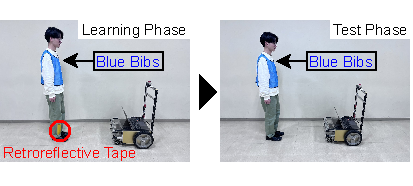
\includegraphics[width=11cm] {images/pdf/RobotGuidance_blue_bibs}
    \captionsetup{justification=raggedright} % キャプションを左寄せに
    \caption{Sequence of the experiment}
    \label{Fig:Sequence of the experiment}
  \end{figure}

\newpage
